\documentclass[a4paper,12pt]{article}
\usepackage{mathrsfs}
\usepackage{geometry}
\usepackage{tcolorbox}
\geometry{a4paper,left=2.5cm,right=2cm,top=2cm,bottom=2cm}

\begin{document}
	\section{Purpose of this DAQ ?}
	I wrote this DAQ in the hope for it to become the (prototype of)
	standard DAQ used by IMP. As far as I learned, by the time this DAQ was
	written, no `standard' DAQ existed in IMP and nobody was working on
	this, even (probably) nobody was thinking about such a thing. This is,
	in my humble opinion, one major thing that we were behind others (e.g.
	GSI, NSCL/FRIB). However, to really develop a universal DAQ applicable
	to many experiments, we may need a whole group to do that. I cannot do
	that on my own. So in this version of DAQ, I kept many thins as simple
	as possible and many things remained unoptimized. The bottom line was to
	make sure that it works and can be easily used by others. How easy could
	it be ? Well, in most cases, one should be able to set it up by just
	clicking mouse and fill in some parameters (like module base addresses)
	without any coding. To that end, one has to use only the modules
	predefined in this DAQ, unsupported modules won't work properly (in
	fact, they won't work at all).
	\section{Overview of this DAQ}
	This DAQ consists of the following parts, see Fig. \ref{fig01}:
	\begin{itemize}
		\item config.py. This is a GUI program (python script) to help user
			create the configuration file used by the DAQ.
		\item frontend. This is the part that communicates with the
			electronics (e.g. VME modules).
		\item evt\_bld. This is the event builder. It grabs data from the
			frontend and build a complete event based on timestamps of the
			fragments readout by frontend.
		\item logger. This program takes data from evt\_bld and records it
			in hard drives.
		\item analyser. This program also takes data from evt\_bld, it
			analysis the events and makes histograms instead of recording
			them.
	\end{itemize}
	The communications between different programs is done via sockets. I
	chose sockets instead of shared memory based on the following
	considerations:
	 i) Different programs do NOT have to run in the same computer. This
	 makes the DAQ more extendable. It also avoids the analyser slowing down
	 the DAQ when it takes too much CPU time.
	 ii) The synchronisation becomes easier because mutex or semaphores are
	 not needed in between programs (although they may still be needed
	 inside a program containing multi threads). Sockets are also easier to
	 handle (as far as I'm concerned).
	 iii) The sockets are of cause slower than shared memory, however, it
	 should not be a problem in most cases.
\begin{figure}
\begin{center}
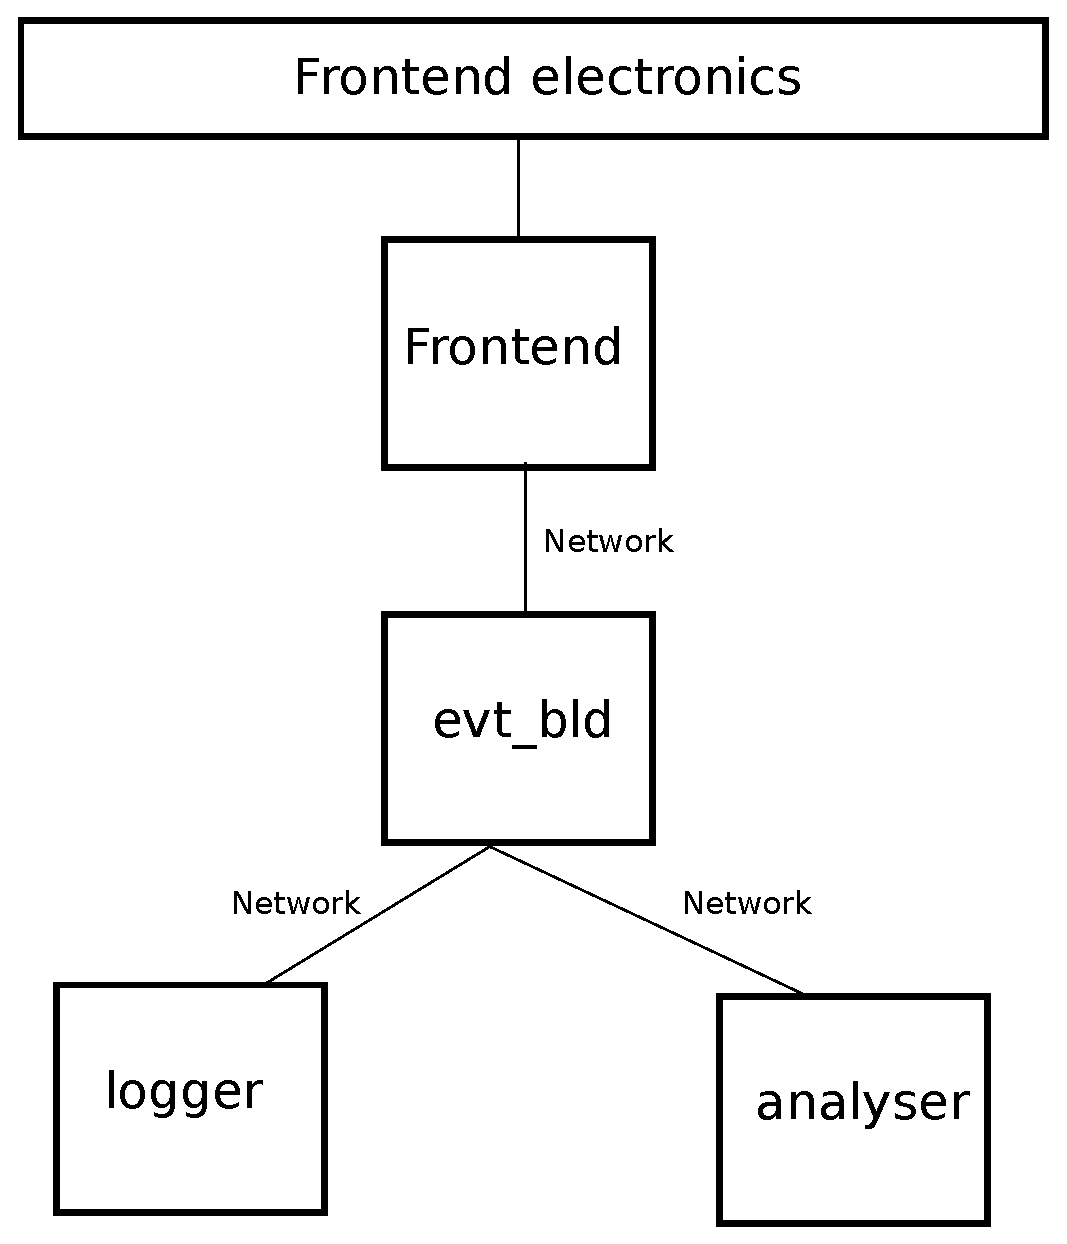
\includegraphics[width=.4\textwidth]{figs/daq_scheme.eps}
    \caption{\label{fig01}Components of the DAQ }
\end{center}
\end{figure}

	 \section{The program `config.py'} This is a helper GUI program written in
	 python to create a
	 configuration file used by the DAQ. This configuration file is a xml
	 file containing the information needed needed by the DAQ. You can run
	 the program without parameters:
	 \begin{tcolorbox}
	 ./config.py
	 \end{tcolorbox}
	 or with parameters:
	 \begin{tcolorbox}
	 ./config.py $<$file name$>$
	 \end{tcolorbox}
	 The difference is that the former one creates a new configuration file
	 from the scratch while the latter one reads in an existing file and
	 allows user to modify it.
	 If you don't feel like using the GUI program, you can also directly
	 modify/create your configuration file using your preferred text editor
	 (e.g. vim, emacs):
	 \begin{tcolorbox}
	 	vim $<$file name$>$
	 \end{tcolorbox}

	 Python 3 is required to run the script. Also because I use tkinter
	 module for GUI programming, you may need to install tk and tcl packages
	 in your system. The tkinter module itself is shipped with python,
	 however, it is just a thin wrapper of the underlying tk/tcl package,
	 you still need to install them. In my system (Arch linux), I did it
	 like:
	 \begin{tcolorbox}
	 	pacman -S tk\\
		pacman -S tcl
	 \end{tcolorbox}


\end{document}
